\documentclass[conference]{IEEEtran}
\IEEEoverridecommandlockouts

\usepackage{cite}
\usepackage{amsmath,amssymb,amsfonts}
\usepackage{graphicx}
\usepackage{textcomp}
\usepackage{xcolor}
\usepackage{booktabs}
\usepackage{multirow}
\usepackage{array}
\usepackage{url}

\def\BibTeX{{\rm B\kern-.05em{\sc i\kern-.025em b}\kern-.08em
    T\kern-.1667em\lower.7ex\hbox{E}\kern-.125emX}}

\begin{document}

\title{Nutrition Grade Prediction from Open Food Facts Data Using Machine Learning and Deep Learning Models}

\author{
\IEEEauthorblockN{Student Name}
\IEEEauthorblockA{\textit{Department Name} \\
\textit{University Name}\\
City, Country \\
student.email@example.com}
}

\maketitle

\begin{abstract}
This study presents a complete machine learning pipeline for predicting the nutrition grade of food products using the Open Food Facts dataset. The original dataset contained a large number of product attributes and missing values; therefore, a preprocessing stage was applied to select nutritionally meaningful features, remove incomplete and duplicate records, and prepare the data for classification. The final dataset contains 14,070 records, 20 features, and five target classes corresponding to nutrition grades. Multiple machine learning algorithms, including Logistic Regression, K-Nearest Neighbors, Decision Tree, Random Forest, and XGBoost, were trained and evaluated. In addition, deep learning models including a Multi-Layer Perceptron, a Deep Neural Network, and a 1D Convolutional Neural Network were considered. The models were compared using accuracy, precision, recall, macro F1-score, and confusion matrices. XGBoost achieved the highest performance among the full-feature models, reaching a test accuracy of 0.9325 and a macro F1-score of 0.9318. After feature selection, XGBoost with the top 10 features achieved 0.9350 accuracy. The results show that gradient boosting is highly effective for structured nutritional tabular data.
\end{abstract}

\begin{IEEEkeywords}
Nutrition grade prediction, Open Food Facts, machine learning, deep learning, XGBoost, classification, food nutrition.
\end{IEEEkeywords}

\section{Introduction}
Nutrition labels provide important information about the health quality of food products. However, manually interpreting nutritional values can be difficult for consumers because products contain many different nutrients, additives, and ingredient-based indicators. Automated prediction of nutrition grade can support food recommendation systems, public health analysis, and consumer decision-making.

In this project, the goal is to predict the nutrition grade of food products from the Open Food Facts dataset. The target variable is \texttt{nutrition\_grade\_fr}, which contains five classes: \texttt{a}, \texttt{b}, \texttt{c}, \texttt{d}, and \texttt{e}. The task is therefore a multi-class classification problem. In the notebook implementation, ordinal encoding was applied as \texttt{a=4}, \texttt{b=3}, \texttt{c=2}, \texttt{d=1}, and \texttt{e=0}. The main contributions of this study are as follows:

\begin{itemize}
    \item A cleaned dataset was created from the original Open Food Facts product data.
    \item Twenty nutritionally meaningful features were selected for model training.
    \item Five machine learning models and three deep learning models were considered.
    \item Model performance was evaluated using accuracy, precision, recall, macro F1-score, and confusion matrices.
    \item The best model was further analyzed with feature selection and SMOTE-based data balancing.
\end{itemize}

\section{Related Work}
Machine learning has been widely applied to food, health, and nutritional classification problems because these domains often contain structured numerical data. Traditional statistical models and linear classifiers can provide interpretable baselines, but they may not capture nonlinear relationships among nutritional values. Tree-based models such as Decision Tree, Random Forest, and gradient boosting methods are commonly used for tabular datasets because they can model nonlinear interactions and handle mixed feature importance patterns.

Previous studies on nutrition and health-related prediction tasks show that ensemble methods often outperform single linear models on structured data. XGBoost, in particular, has been successful in many tabular classification tasks because it combines multiple weak learners through gradient boosting and includes regularization mechanisms. Deep learning models such as Multi-Layer Perceptrons and Deep Neural Networks can also learn nonlinear relationships, but they usually require larger datasets and careful regularization to outperform tree-based methods on tabular data. Based on these observations, this study compares both classical machine learning and deep learning approaches for nutrition grade prediction.

\section{Methodology}
The proposed methodology consists of data collection, exploratory data analysis, data preprocessing, model development, model evaluation, feature selection, class balancing, and final comparison. The overall goal is to build a reliable prediction system that classifies food products into one of five nutrition grade categories using selected nutritional and ingredient-based features.

\subsection{Data Collection}
The original Open Food Facts dataset contains a large number of food product records and nutritional attributes. Since many products have incomplete nutrition information, data cleaning was necessary before training machine learning models.

After preprocessing, the final dataset contains 14,070 records, 20 input features, and one target variable. The target variable has five classes. Table~\ref{tab:dataset-summary} summarizes the final dataset.

\begin{table}[htbp]
\caption{Final Dataset Summary}
\begin{center}
\begin{tabular}{lr}
\toprule
\textbf{Property} & \textbf{Value} \\
\midrule
Number of records & 14,070 \\
Number of features & 20 \\
Target classes & 5 \\
Missing values & 0 \\
Duplicate records & 0 \\
\bottomrule
\end{tabular}
\label{tab:dataset-summary}
\end{center}
\end{table}

The class distribution is shown in Table~\ref{tab:class-distribution}. The classes \texttt{a}, \texttt{b}, \texttt{c}, and \texttt{d} are relatively balanced, while class \texttt{e} contains fewer samples.

\begin{table}[htbp]
\caption{Target Class Distribution}
\begin{center}
\begin{tabular}{lrr}
\toprule
\textbf{Class} & \textbf{Count} & \textbf{Percentage} \\
\midrule
a & 3,188 & 22.66\% \\
b & 3,337 & 23.72\% \\
c & 3,142 & 22.33\% \\
d & 3,297 & 23.43\% \\
e & 1,106 & 7.86\% \\
\bottomrule
\end{tabular}
\label{tab:class-distribution}
\end{center}
\end{table}

\begin{figure}[htbp]
\centerline{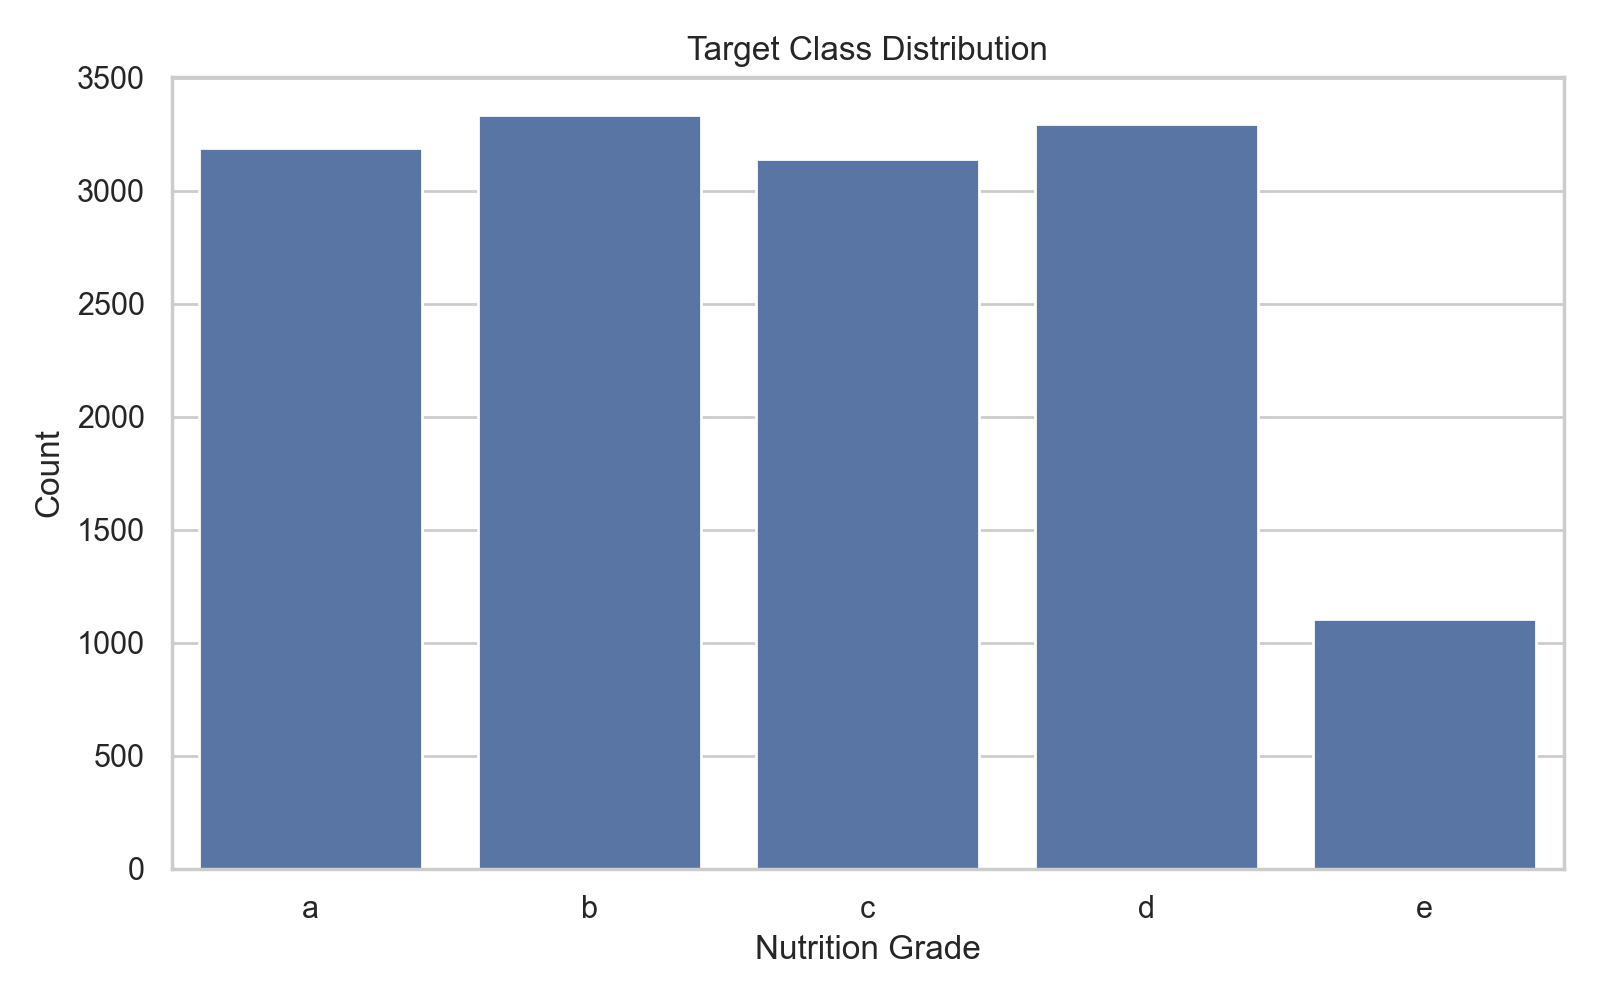
\includegraphics[width=\columnwidth]{figures/target_distribution.png}}
\caption{Target class distribution in the cleaned dataset.}
\label{fig:target-distribution}
\end{figure}

\subsection{Data Analysis}
Exploratory data analysis was conducted to understand the distribution of the target classes, missing values, zero values, feature statistics, and feature correlations. The analysis showed that the dataset is suitable for multi-class classification after cleaning, but it also revealed class imbalance in the minority class \texttt{e}. Feature correlation analysis also identified a strong correlation between \texttt{salt\_100g} and \texttt{sodium\_100g}.

\subsection{Data Preprocessing}
\subsubsection{Handling Missing Data}
The original dataset contained many missing values because not all food products had complete nutritional information. Missing values were handled by removing records with missing values in the selected features or the target variable. After preprocessing, the final dataset contained no missing values. Since all selected records were complete, no imputation method such as mean, median, or mode replacement was required.

\subsubsection{Duplicate Removal}
Duplicate records were removed to reduce data leakage and prevent the models from learning repeated product patterns. After duplicate removal, the final dataset contained 14,070 unique records.

\subsubsection{Zero Value Analysis}
Some features contained many zero values. For example, trans fat and palm oil indicators were zero for most products. This is not necessarily incorrect, because many products do not contain trans fat or palm oil. However, records with effectively empty nutrition tables were removed during preprocessing. The final dataset contains no rows where all nutritional features are zero.

\begin{figure}[htbp]
\centerline{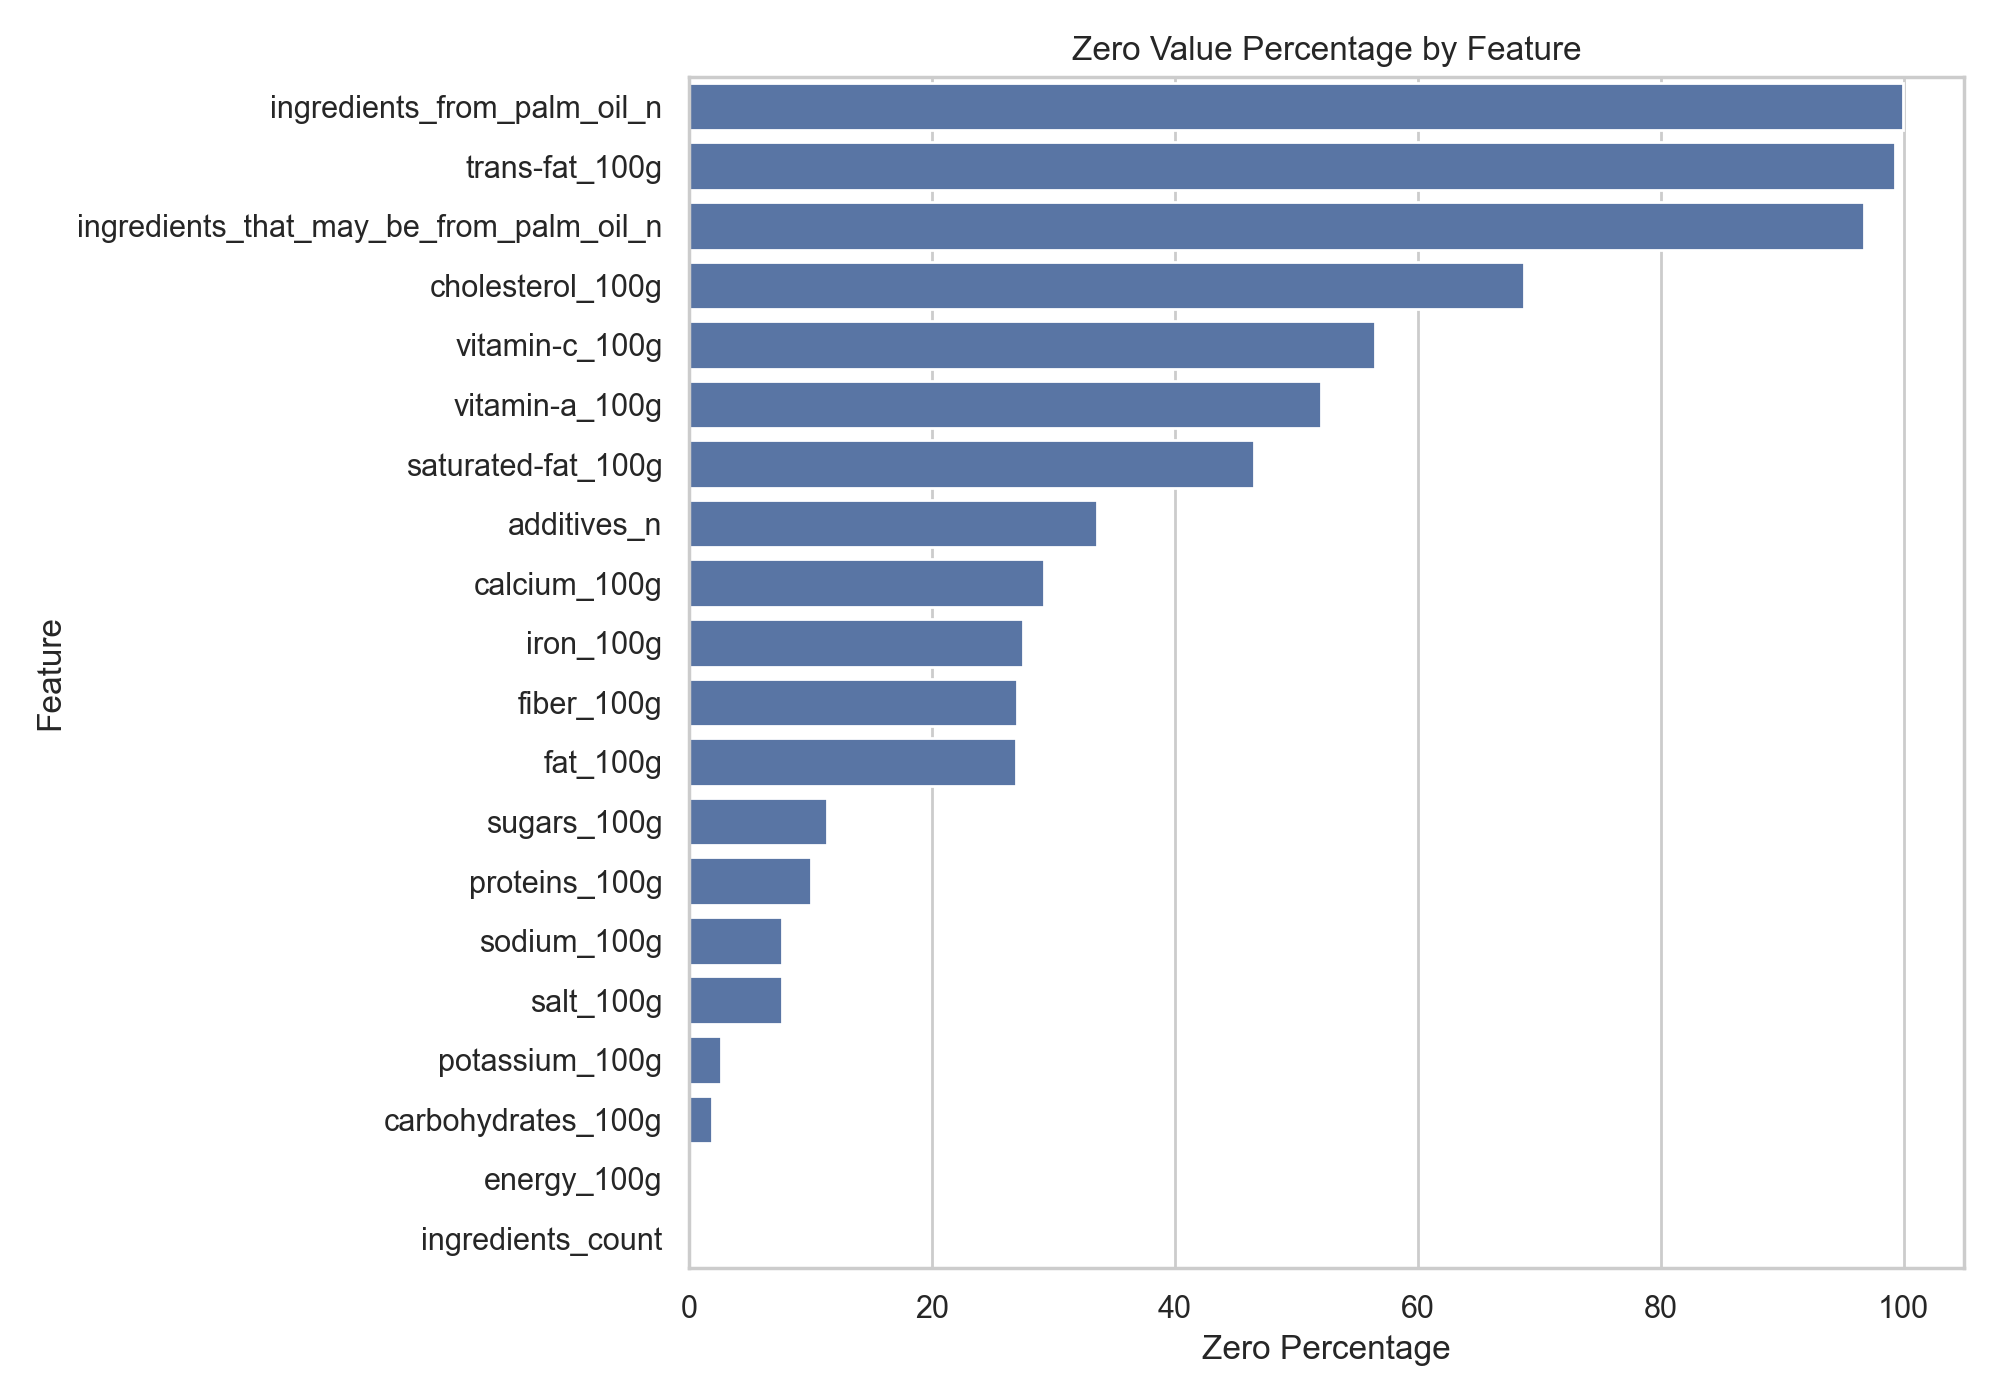
\includegraphics[width=\columnwidth]{figures/zero_value_distribution.png}}
\caption{Zero value percentage by feature.}
\label{fig:zero-values}
\end{figure}

\subsubsection{Data Standardization}
Standardization was applied to scale-sensitive models such as Logistic Regression, K-Nearest Neighbors, and neural network models. The scaler was fitted only on the training data and then applied to the test data to avoid data leakage. Tree-based models such as Decision Tree, Random Forest, and XGBoost were trained using the original feature values because they are not sensitive to feature scale.

\section{Feature Analysis and Correlation}
The selected 20 features include energy, macronutrients, salt-related values, micronutrients, additives, palm oil indicators, and ingredient count. These features were selected because they are nutritionally meaningful and relevant to the prediction of nutrition grade.

The selected features are:
\begin{itemize}
    \item \texttt{energy\_100g}, \texttt{fat\_100g}, \texttt{saturated-fat\_100g}
    \item \texttt{carbohydrates\_100g}, \texttt{sugars\_100g}, \texttt{fiber\_100g}, \texttt{proteins\_100g}
    \item \texttt{salt\_100g}, \texttt{sodium\_100g}, \texttt{trans-fat\_100g}, \texttt{cholesterol\_100g}
    \item \texttt{calcium\_100g}, \texttt{iron\_100g}, \texttt{potassium\_100g}
    \item \texttt{vitamin-c\_100g}, \texttt{vitamin-a\_100g}
    \item \texttt{additives\_n}, \texttt{ingredients\_from\_palm\_oil\_n}, \texttt{ingredients\_that\_may\_be\_from\_palm\_oil\_n}, \texttt{ingredients\_count}
\end{itemize}

Correlation analysis showed that most features did not have extreme correlation. However, \texttt{salt\_100g} and \texttt{sodium\_100g} had a correlation of 1.0000 because salt and sodium are mathematically related. Both were kept because the project required 20 features and both are nutritionally meaningful.

\begin{table}[htbp]
\caption{Notable Feature Correlations}
\begin{center}
\begin{tabular}{llr}
\toprule
\textbf{Feature 1} & \textbf{Feature 2} & \textbf{Correlation} \\
\midrule
salt\_100g & sodium\_100g & 1.0000 \\
energy\_100g & fat\_100g & 0.7888 \\
additives\_n & ingredients\_count & 0.7467 \\
energy\_100g & carbohydrates\_100g & 0.7103 \\
fat\_100g & saturated-fat\_100g & 0.6692 \\
carbohydrates\_100g & sugars\_100g & 0.5739 \\
\bottomrule
\end{tabular}
\label{tab:feature-correlation}
\end{center}
\end{table}

\begin{figure}[htbp]
\centerline{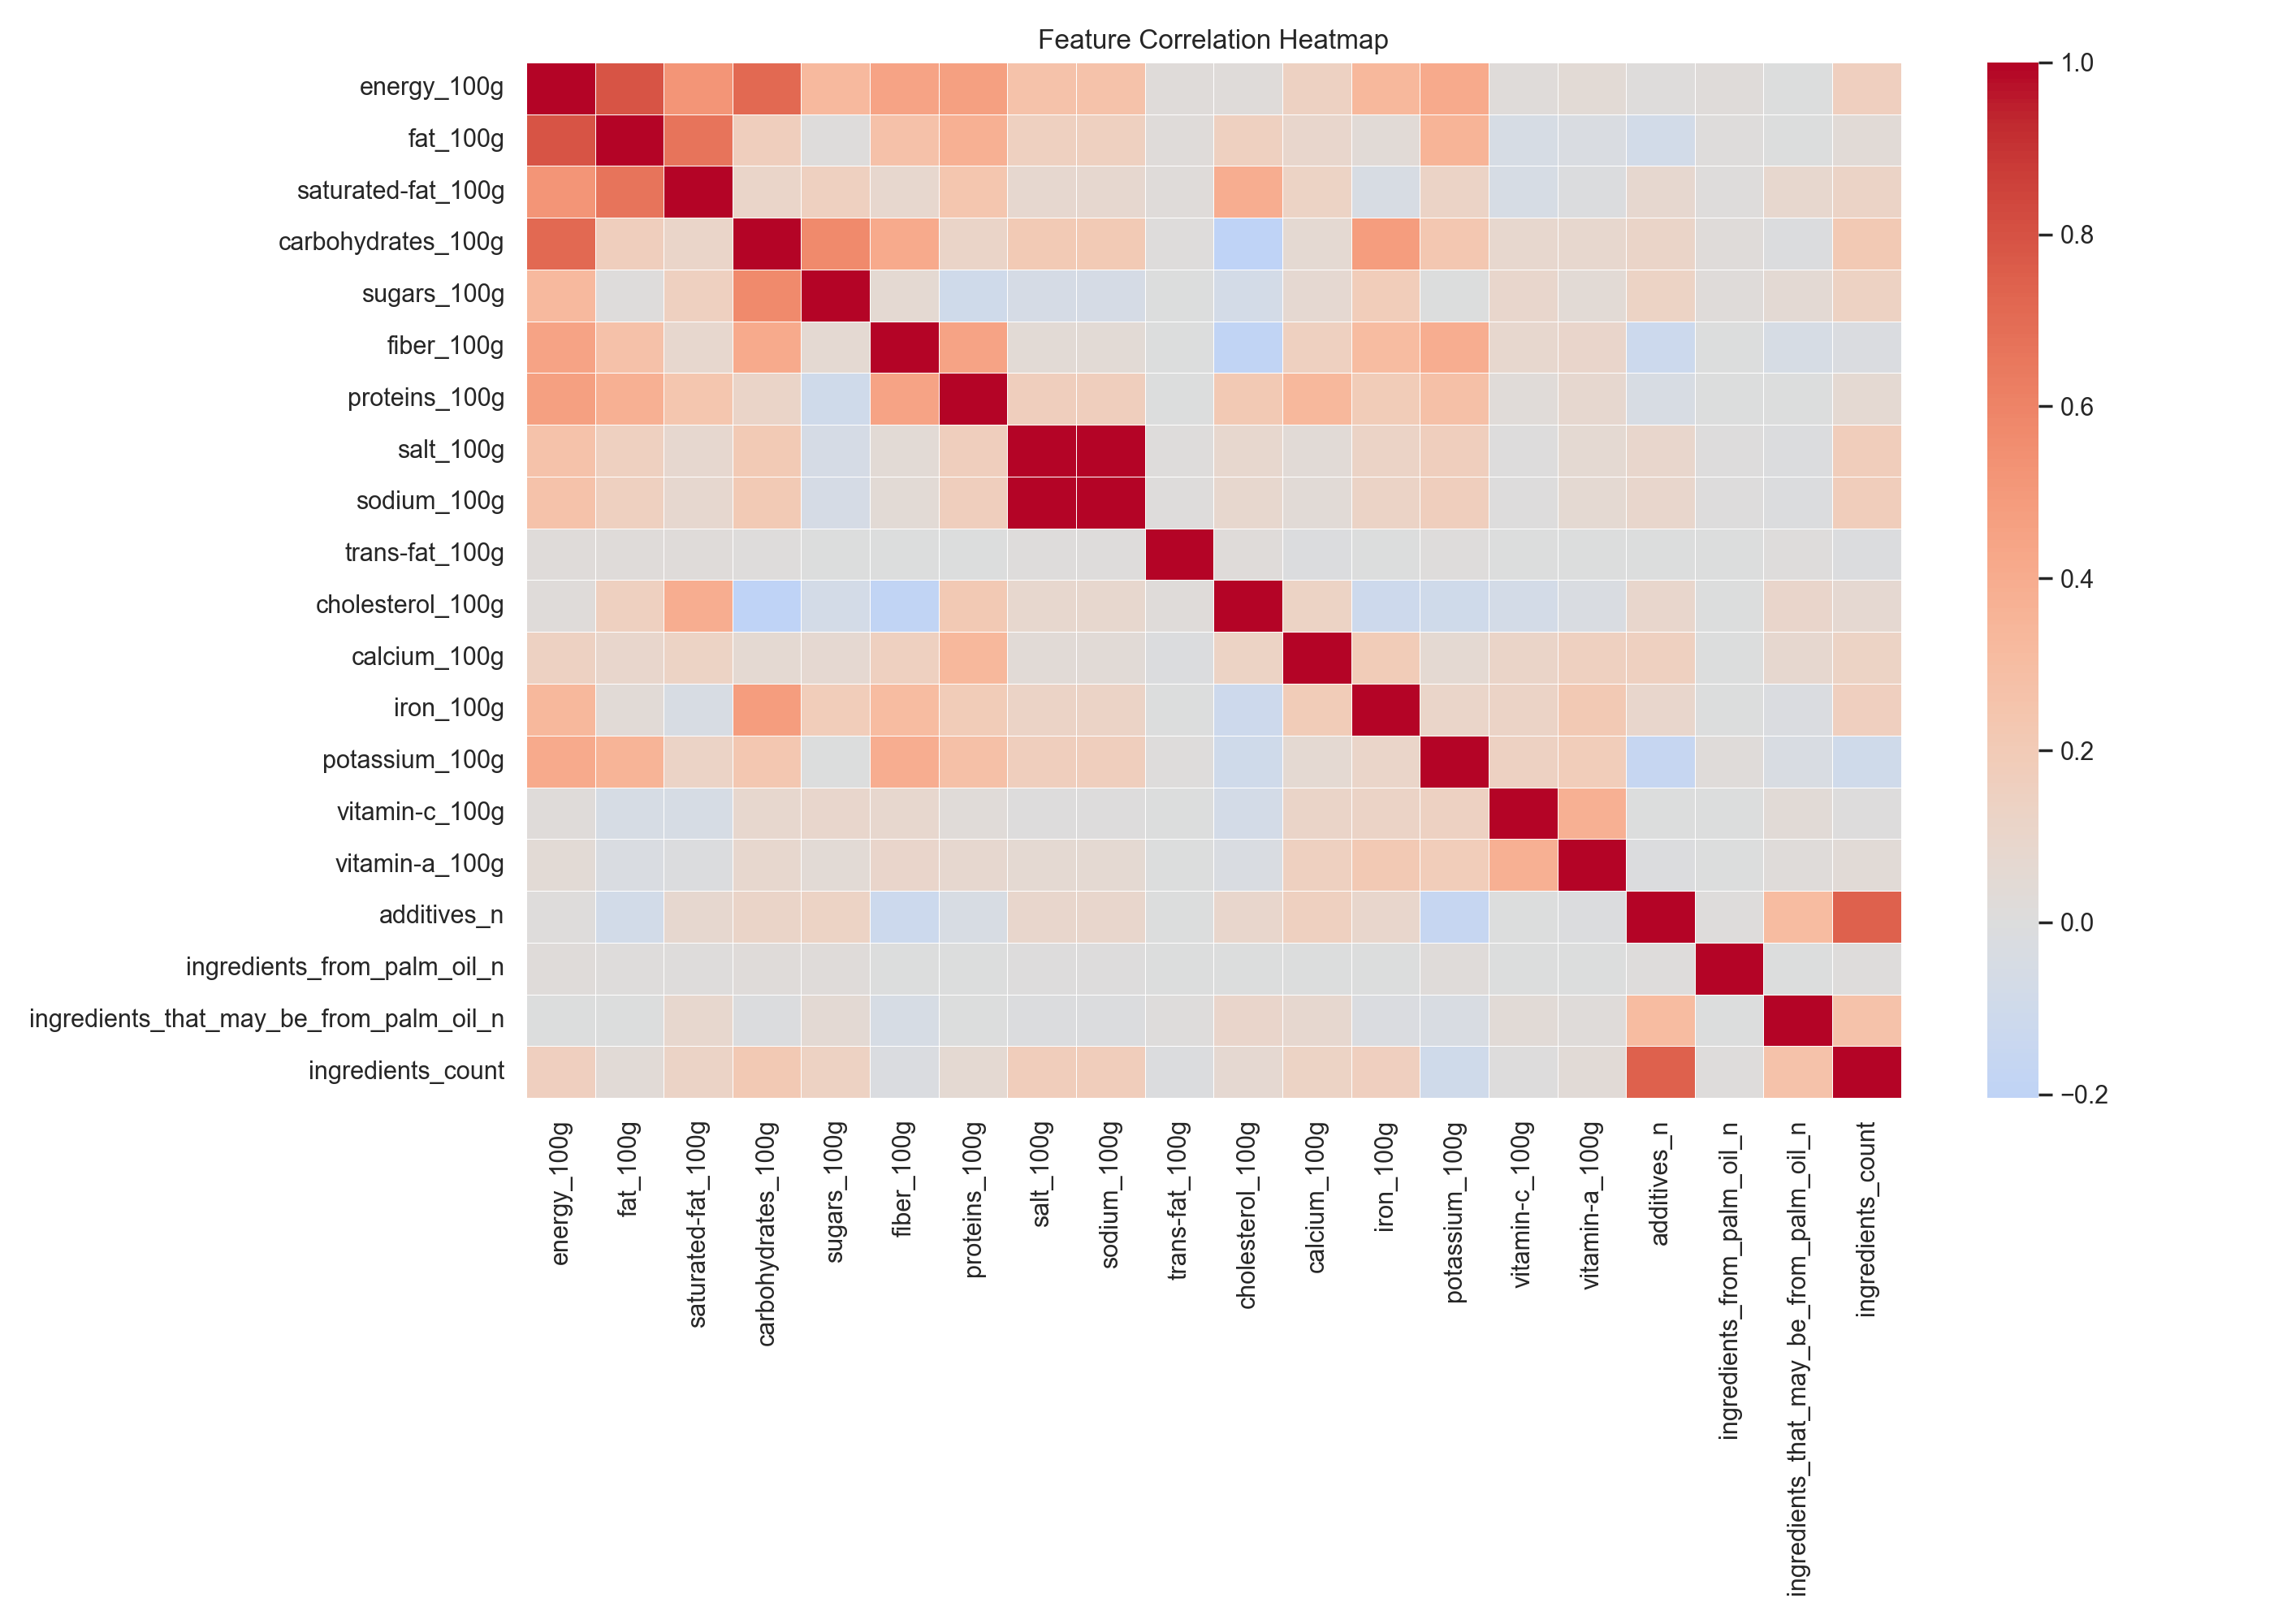
\includegraphics[width=\columnwidth]{figures/feature_correlation_heatmap.png}}
\caption{Feature correlation heatmap.}
\label{fig:correlation-heatmap}
\end{figure}

\section{Machine Learning Models}
Five machine learning models were used: Logistic Regression, K-Nearest Neighbors, Decision Tree, Random Forest, and XGBoost.

\subsection{Logistic Regression}
Logistic Regression was used as a linear baseline model. StandardScaler was applied before training. The model was trained with \texttt{max\_iter=5000}, \texttt{class\_weight=balanced}, and \texttt{random\_state=42}.

\subsection{K-Nearest Neighbors}
KNN was trained using standardized features. Cross-validation was used to select the best hyperparameters. The best KNN model used Manhattan distance, \texttt{n\_neighbors=5}, and distance-based weighting. The best 5-fold cross-validation macro F1-score was 0.8611.

\subsection{Decision Tree}
Decision Tree was trained using entropy as the splitting criterion. The final notebook model used \texttt{max\_depth=12}, \texttt{min\_samples\_leaf=5}, \texttt{min\_samples\_split=2}, and \texttt{class\_weight=balanced}. Entropy was selected because it uses information gain for node splitting.

\subsection{Random Forest}
Random Forest was trained as an ensemble of decision trees. To reduce overfitting, the final notebook model used \texttt{n\_estimators=200}, \texttt{criterion=entropy}, \texttt{max\_depth=12}, \texttt{min\_samples\_split=5}, \texttt{min\_samples\_leaf=10}, and \texttt{class\_weight=balanced}.

\subsection{XGBoost}
XGBoost was used as the main gradient boosting model. The model used \texttt{n\_estimators=300}, \texttt{max\_depth=5}, \texttt{learning\_rate=0.05}, \texttt{subsample=0.8}, \texttt{colsample\_bytree=0.8}, \texttt{objective=multi:softprob}, and \texttt{eval\_metric=mlogloss}. Balanced sample weights were used to reduce the effect of class imbalance.

\section{Deep Learning Models}
Three deep learning architectures were considered: MLP, DNN, and 1D CNN.

\subsection{Multi-Layer Perceptron}
The MLP model consisted of dense layers with ReLU activation and dropout regularization. The output layer used softmax activation for five-class classification. Early stopping was used to reduce overfitting.

\subsection{Deep Neural Network}
The DNN model was designed as a deeper version of the MLP. It included multiple dense layers, Batch Normalization, and Dropout layers. This architecture was used to test whether a deeper network could improve classification performance.

\subsection{1D Convolutional Neural Network}
The 1D CNN model reshaped the 20 numerical input features into a one-dimensional sequence with one channel. Conv1D layers were then used to learn local patterns among nutritional features.

\section{Model Evaluation}
The models were evaluated using accuracy, precision, recall, macro F1-score, and confusion matrices. Macro F1-score was emphasized because the class distribution was not perfectly balanced, especially for class \texttt{e}.

\begin{table*}[htbp]
\caption{Model Performance Comparison}
\begin{center}
\begin{tabular}{lrrrr}
\toprule
\textbf{Model} & \textbf{Accuracy} & \textbf{Precision} & \textbf{Recall} & \textbf{Macro F1-score} \\
\midrule
Logistic Regression & 0.7591 & 0.7574 & 0.7763 & 0.7642 \\
KNN with CV & 0.8547 & 0.8608 & 0.8514 & 0.8556 \\
Decision Tree & 0.8834 & 0.8770 & 0.8863 & 0.8812 \\
Random Forest & 0.8842 & 0.8843 & 0.8860 & 0.8849 \\
XGBoost & 0.9325 & 0.9330 & 0.9308 & 0.9318 \\
MLP & 0.9112 & 0.9083 & 0.9166 & 0.9115 \\
DNN & 0.8952 & 0.8919 & 0.9022 & 0.8962 \\
1D CNN & 0.8923 & 0.8928 & 0.8914 & 0.8919 \\
\bottomrule
\end{tabular}
\label{tab:model-comparison}
\end{center}
\end{table*}

Among the evaluated full-feature models, XGBoost achieved the highest test performance with an accuracy of 0.9325 and a macro F1-score of 0.9318. The MLP model was the strongest deep learning model, achieving 0.9112 accuracy and 0.9115 macro F1-score. Logistic Regression had the lowest performance, indicating that the relationship between nutritional features and nutrition grade is nonlinear.

\subsection{Confusion Matrix Analysis}
Confusion matrices were generated during experimentation to inspect class-level prediction behavior. To keep the final conference-style report concise, only the confusion matrix comparison required for the SMOTE experiment is included in the main text.

\section{SMOTE-Based Data Balancing}
Since class \texttt{e} had fewer samples than the other classes, Synthetic Minority Oversampling Technique (SMOTE) was used for data balancing on the best accuracy model, XGBoost. SMOTE was applied only to the training data, while the test set remained unchanged and contained only real data. This prevents data leakage and ensures that final evaluation is performed on real records.

The before-SMOTE XGBoost model was trained using class-balanced sample weights. The after-SMOTE model was trained on the SMOTE-balanced training set. Confusion matrices before and after SMOTE were compared to determine whether minority class prediction improved.

\begin{table}[htbp]
\caption{XGBoost Before and After SMOTE}
\begin{center}
\begin{tabular}{lrrrr}
\toprule
\textbf{Setting} & \textbf{Acc.} & \textbf{Prec.} & \textbf{Rec.} & \textbf{F1} \\
\midrule
Before SMOTE & 0.9325 & 0.9330 & 0.9308 & 0.9318 \\
After SMOTE & 0.9314 & 0.9316 & 0.9299 & 0.9306 \\
\bottomrule
\end{tabular}
\label{tab:smote-results}
\end{center}
\end{table}

\section{Feature Selection and Reduction}
Feature selection was performed using XGBoost feature importance scores. First, the model was trained using all 20 features. Then, the top 10 most important features were selected and the model was retrained using only those selected features. This comparison shows whether a smaller feature subset can maintain similar performance.

The top features identified by XGBoost included \texttt{saturated-fat\_100g}, \texttt{energy\_100g}, \texttt{sugars\_100g}, \texttt{proteins\_100g}, \texttt{fiber\_100g}, \texttt{salt\_100g}, \texttt{sodium\_100g}, \texttt{fat\_100g}, \texttt{carbohydrates\_100g}, and \texttt{ingredients\_from\_palm\_oil\_n}.

\begin{table}[htbp]
\caption{Feature Selection Comparison with XGBoost}
\begin{center}
\begin{tabular}{lrrrr}
\toprule
\textbf{Feature Set} & \textbf{No.} & \textbf{Acc.} & \textbf{Rec.} & \textbf{F1} \\
\midrule
All features & 20 & 0.9325 & 0.9308 & 0.9318 \\
Top 10 features & 10 & 0.9350 & 0.9340 & 0.9340 \\
\bottomrule
\end{tabular}
\label{tab:feature-selection}
\end{center}
\end{table}

\begin{figure}[htbp]
\centerline{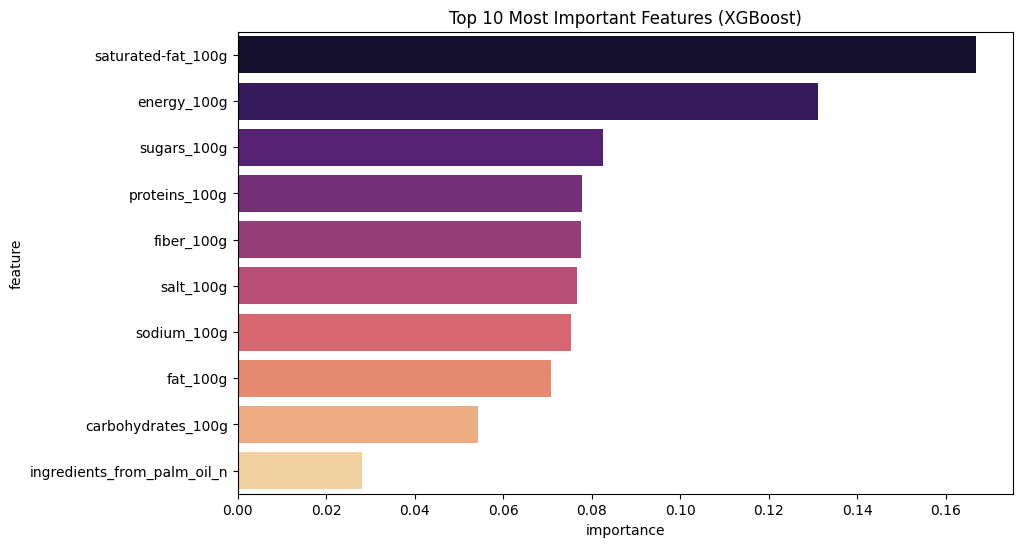
\includegraphics[width=\columnwidth]{figures/xgboost_top10_feature_importance.png}}
\caption{Top 10 feature importances obtained from the XGBoost model.}
\label{fig:xgb-top10-importance}
\end{figure}

\section{Training and Runtime Analysis}
Training time and runtime for one record were measured using the 80\%-20\% train-test split. Training time represents the duration required to fit the model, while single-record runtime represents the prediction time for one sample. For deep learning models, training time was taken from the model training history and prediction runtime was measured on a single scaled test record.

\begin{table}[htbp]
\caption{Training Time and Single Record Runtime}
\begin{center}
\begin{tabular}{lll}
\toprule
\textbf{Model} & \textbf{Training Time (s)} & \textbf{One Record Runtime (s)} \\
\midrule
Logistic Regression & 0.7404 & 0.000156 \\
KNN Optimized & 0.0027 & 0.001129 \\
Decision Tree & 0.1654 & 0.001031 \\
Random Forest & 4.9080 & 0.055375 \\
XGBoost Full & 4.8410 & 0.004218 \\
XGBoost Top 10 & 2.5713 & 0.001816 \\
MLP & 60.7906 & 0.296751 \\
DNN & 40.8359 & 0.392009 \\
1D CNN & 43.9195 & 0.442575 \\
\bottomrule
\end{tabular}
\label{tab:runtime}
\end{center}
\end{table}

\section{Iterative Enhancement of Deep Learning Models}
For deep learning models, iterative enhancement was performed by modifying model architecture and training strategies. The improvements included adding more dense layers, using dropout, applying Batch Normalization, using class weights, and adding early stopping. These steps were used to improve validation performance and reduce overfitting.

\begin{table}[htbp]
\caption{Iterative Enhancement for Deep Learning}
\begin{center}
\begin{tabular}{llrr}
\toprule
\textbf{Version} & \textbf{Enhancement} & \textbf{Acc.} & \textbf{F1} \\
\midrule
MLP & Dense layers, dropout, early stopping, class weights & 0.9112 & 0.9115 \\
DNN & Added depth and Batch Normalization & 0.8952 & 0.8962 \\
1D CNN & Added Conv1D layers & 0.8923 & 0.8919 \\
\bottomrule
\end{tabular}
\label{tab:dl-enhancement}
\end{center}
\end{table}

\section{Discussion}
The experimental results show that gradient boosting is highly effective for the selected nutrition grade prediction task. XGBoost achieved the best full-feature performance, and the feature-selected XGBoost model achieved the highest overall accuracy in the notebook. This is expected because the dataset is structured tabular data with a moderate number of numerical features. Gradient boosting methods are known to perform strongly on this type of data.

The MLP model achieved a strong test accuracy of 0.9112, but it did not outperform XGBoost. This result is reasonable because neural networks often require larger and more complex datasets to outperform tree-based models on tabular data. Logistic Regression had the lowest performance, which suggests that the relationship between nutritional features and nutrition grade is not purely linear.

The correlation analysis showed that \texttt{salt\_100g} and \texttt{sodium\_100g} are highly correlated. Although this may introduce redundancy, both features were retained to satisfy the 20-feature requirement and because both are nutritionally meaningful. Feature selection analysis was also included to evaluate whether a reduced feature set could maintain strong performance.

\section{Conclusion}
This project developed a complete machine learning and deep learning pipeline for nutrition grade prediction using the Open Food Facts dataset. After preprocessing, the final dataset contained 14,070 records, 20 features, no missing values, and no duplicate records. Multiple algorithms were trained and evaluated. XGBoost achieved the best full-feature performance with a test accuracy of 0.9325 and a macro F1-score of 0.9318. After feature selection, XGBoost with the top 10 features achieved 0.9350 accuracy. The results indicate that gradient boosting methods are particularly suitable for structured nutritional data. Future work may include additional feature engineering, larger datasets, and deployment of the best model through a Streamlit-based user interface for real-time nutrition grade prediction.

\begin{thebibliography}{00}
\bibitem{b1} Open Food Facts, ``Open Food Facts database,'' Accessed: 2026. [Online]. Available: \url{https://world.openfoodfacts.org/data}
\bibitem{b2} T. Chen and C. Guestrin, ``XGBoost: A scalable tree boosting system,'' in \textit{Proceedings of the 22nd ACM SIGKDD International Conference on Knowledge Discovery and Data Mining}, 2016, pp. 785--794.
\bibitem{b3} N. V. Chawla, K. W. Bowyer, L. O. Hall, and W. P. Kegelmeyer, ``SMOTE: Synthetic Minority Over-sampling Technique,'' \textit{Journal of Artificial Intelligence Research}, vol. 16, pp. 321--357, 2002.
\bibitem{b4} F. Pedregosa et al., ``Scikit-learn: Machine learning in Python,'' \textit{Journal of Machine Learning Research}, vol. 12, pp. 2825--2830, 2011.
\bibitem{b5} M. Abadi et al., ``TensorFlow: Large-scale machine learning on heterogeneous systems,'' 2015. [Online]. Available: \url{https://www.tensorflow.org/}
\end{thebibliography}

\end{document}
